\documentclass{40k}

\usepackage{pdflscape}
\usepackage{enumitem}

%%----------------------------------------------------------------------
%% Decorations
%%----------------------------------------------------------------------

\newcommand{\teaser}[1]{\centerline{\emph{#1}}}

%%----------------------------------------------------------------------
%% Deployment Zones
%%----------------------------------------------------------------------

\newenvironment{tablesetup}
{\missionheading{Table Setup}}
{}

\newcommand{\dawnofwar}%
{Deployment zones are \textbf{Dawn of War}, as on page~131 of the
\emph{Warhammer 40,000} rulebook (12'' long edges).}

\newcommand{\hammerandanvil}%
{Deployment zones are \textbf{Hammer and Anvil}, as defined on
  page~131 of the main rulebook (24'' short edges).}

\newcommand{\vanguardstrike}%
{Deployment zones are \textbf{Vanguard Strike}, as defined on page~131
  of the main \emph{Warhammer 40,000} rulebook.  Vanguard Strike may
  be approximated by deploying within a 33.5'' x 50'' table corner
  triangle.  The player that wins the zone roll off may pick any of
  the four corners, and the other player takes that diagonally
  opposite.}

\newcommand{\quartered}%
{Deployment zones are the rectangles in each table corner~12'' in from
  the long edge and~24'' in from the short edges.  The player that
  wins the zone roll off picks either pair of \emph{diagonally
    opposite} corners as their deployment zone and a long table edge
  as their player edge.  The other player takes the other pair of
  diagonally opposite corners and opposite long edge.}

%%----------------------------------------------------------------------
%% Mission Rules
%%----------------------------------------------------------------------

\newenvironment{missionrules}
{
\missionheading{Mission Specific Rules}

The following mission specific rules apply, in addition to those
applied to all missions in this packet.
}
{
}

\newcommand{\nightfighting}%
{\missionsubheading{Night Fighting.}  If either player opts for Night
  Fighting before any deployment begins, on a single D6 of 4+ all
  units have Stealth throughout Turn 1.}

\newcommand{\nightfalls}%
{\missionsubheading{Night Falls.}  If either player opts for Night
  Falls before any deployment begins, on a single~D6 of~4+ all units
  except superheavy vehicles and gargantuan creatures have Stealth
  throughout Turns~5,~6, and~7.}


%%----------------------------------------------------------------------
%% Scoring
%%----------------------------------------------------------------------

\newenvironment{scoring}{
\missionheading{Scoring}

% This mission is scored by objectives achieved, as follows.
}
{

\missionsubheading{Secondary Objectives.}

After deployment, both players simultaneously choose and reveal a
personal secondary objective from the options available for their
campaign goal.  Any necessary selections are also chosen and revealed
then unless noted otherwise.  \underline{No more than~6 victory points
  may be earned via these.}

\missionsubheading{Tertiary Objectives.}  As given in the overall
Common Rules section of this packet.
}

\newenvironment{primaries}
{
\missionsubheading{Primary Objectives.}  
}
{}


%%----------------------------------------------------------------------
%% Secondaries
%%----------------------------------------------------------------------

\newenvironment{secondaries}
{
}
{
}

\newcommand{\seekanddestroy}%
{\item \textit{Seek and Destroy.}  Choose and declare a Battlefield
  Role other than Troop.  Score~2 victory points for each enemy unit
  of this role completely destroyed or falling back at the end of the
  game.}

\newcommand{\securepositions}%
{\item \textit{Secure Positions.}  For each table quadrant, secretly
  select a terrain piece at least~50\% inside it, recording your
  selections unambiguously.  Reveal these at game end and score~2
  victory points for each that you control, treating them as objective
  markers.  Note that this means a single unit cannot claim both a
  primary objective marker and a terrain piece, nor multiple pieces
  simultaneously.}

\newcommand{\breachpoints}%
{\item \textit{Breach Points.}  Choose two terrain pieces at least
  partially in the opposing deployment zone.  Do not declare these
  now, but do secretly record your selection unambiguously!  Reveal
  these at game end and score~3 victory points for each piece that you
  control, treating them as objective markers.  Note that this means a
  single unit cannot claim both a primary objective marker and a
  terrain piece simultaneously.}

\newcommand{\seizeground}%
{\item \textit{Seize Ground.}  Choose two terrain pieces not in your
  deployment zone.  Do not declare these now, but do secretly record
  your selection unambiguously!  Reveal these at game end and score~3
  victory points for each piece that you control, treating them as
  objective markers.  Note that this means a single unit cannot claim
  both a primary objective marker and a terrain piece simultaneously.}

\newcommand{\reconnaissance}%
{\item \textit{Reconnaissance.}  At game end, score~2 victory points
  for each friendly scoring unit with the Scout or Infiltrate USR
  completely within 12'' of your opponent's table edge.}

\newcommand{\meatgrinder}%
{\item \textit{Meatgrinder.}  Score~1 victory point for each opposing
  Troop unit completely destroyed or falling back at the end of the
  game.}

\newcommand{\hullbreaker}%
{\item \textit{Hullbreaker.}  Score~1 victory point for each opposing
  vehicle completely destroyed or monstrous creature removed as a
  casualty.}

\newcommand{\assassination}%
{\item \textit{Assassination.}  Score~1 victory point for each
  opposing character model removed as a casualty or falling back at
  the end of the game.  Note that this is not limited to just
  independent characters.}

\newcommand{\interrogation}%
{\item \textit{Interrogation.}  Score~1 victory point for each
  opposing character model removed as a casualty in close combat.  In
  addition, whenever an opposing character model is removed as a
  casualty by any means, put a secondary objective marker in its
  place.  You score~1 victory point for each such marker controlled at
  game end.  Note that neither of these criteria are limited to just
  independent characters.}

\newcommand{\frontline}%
{\item \textit{Frontline.} Place three secondary objective markers
  within~18'' of your opponent's table edge, 6'' from all table edges
  and 12'' from all objective markers or as far apart as possible. At
  game end, score 3 victory points for each of these markers you
  control.}

\newcommand{\controlthefield}%
{\item \textit{Control the Field.}  Each table quarter in which you
  have a scoring unit and your opponent does not, or you have an
  Objective Secured Unit and your opponent does not, is worth 2
  victory points at game end.}

\newcommand{\breaktheirback}%
{\item \textit{Break Their Back.}  At game end, each enemy unit that
  has been eliminated, is falling back, or has at most~25\% of its
  starting models remaining is broken.  Earn~2 victory points per
  quartile if at least 25\%, 50\%, and 75\% of your opponent's army by
  units is broken.}

\newcommand{\stalwart}%
{\item \textit{Stalwart.} Score~2 victory points for each objective
  marker held at game end.}

\newcommand{\holdthefield}%
{\item \textit{Hold The Field.} Score~2 victory points for every~2
  objective markers held at game end.}

\newcommand{\overrun}%
{\item \textit{Overrun.}  At game end, count how many scoring units
  you have at least partially within your opponent's half of the
  table, and how many scoring units your opponent has at least
  partially within your half of the table.  If your number is higher,
  score~2 victory points for each point of difference.}

\newcommand{\majoritycontrol}%
{\item \textit{Majority Control.}  At the end of each game turn,
  score~1 victory point if you control more objective markers than
  your opponent.  Score an additional point if you control more than
  half of the markers.}


%%----------------------------------------------------------------------
%% Maelstrom
%%----------------------------------------------------------------------

\newcommand{\maelstrom}{%
  \missionsubheading{The Storm.}%
  At the start of each player turn, the active player draws tactical
  objectives until they have as many in play as the current turn
  number.

  \maelstromrules
}

\newcommand{\standingorders}{%
  \missionsubheading{Standing Orders.}%
  At the start of your turns, draw tactical
  objectives until you have a total of six in play.

  \maelstromrules
}

\newcommand{\maelstromrules}{%
  \missionsubheading{Maelstrom.}%
  To draw a tactical objective, roll a~D66 and consult your tactical
  objective table, attached at the end of this mission packet.  If
  that objective is already in play for you, has been achieved, or is
  scratched off, roll again.  Similarly, if that objective would be
  provably impossible to score, e.g., your opponent has no characters
  remaining, roll again.  Once a valid objective has been rolled, mark
  it as in play.

  Targets cannot be nominated or chosen for a tactical objective
  marked with a $\dagger$ that have already been chosen for a
  $\dagger$ objective you have in play.

  \smallskip%
  At the end of your turns, check the requirements for each tactical
  objective you have in play.  For each fixed-value objective met,
  mark it as achieved and score the associated value in \emph{mission
    points} (n.b.: not \emph{victory points}).  Tactical objectives
  with a value of X may be kept in play as long as you wish.  At the
  end of any of your turns while in play they may be marked as
  achieved and scored as indicated.  Once achieved, objectives are no
  longer considered in play and cannot be put in play or scored again.

  Multiple objectives can be scored in a turn, caveat that you cannot
  achieve multiple tactical objectives with the same exact title in
  the same turn using the same marker(s) or unit(s).  E.g., to score
  both Storm objectives at once, you would need to simultaneously
  control two separate markers in the enemy deployment zone.

  At the end of your turn you may scratch out one of your tactical
  objectives in play to remove it from play.

  \smallskip%
  Tactical objectives in play, achieved, and scratched out are not
  secret.}

\newcommand{\maelstromscoring}
{At game end, compare mission points earned through tactical
objectives achieved and award victory points to the higher and lower
scorer as follows:

%\definecolor{Gray}{gray}{0.9}
%\definecolor{DGray}{gray}{0.75}
\newcolumntype{a}{>{\columncolor{gray!25}}c}
\newcolumntype{b}{>{\columncolor{gray!50}}r}
\bigskip\centerline{\setlength{\tabcolsep}{12pt}%
\begin{tabular}{|b|c|a|c|a|c|a|}
\hline
{\bf Difference}     & 0     & 1--2  & 3--4  & 5--6  & 7     & 8+\\
{\bf Victory Points} & 4 / 4 & 5 / 4 & 6 / 3 & 7 / 2 & 8 / 1 & 9 / 0\\
\hline
\end{tabular}}}


%%----------------------------------------------------------------------
%%----------------------------------------------------------------------
\begin{document}


%%----------------------------------------------------------------------
%%----------------------------------------------------------------------
%%----------------------------------------------------------------------
%%----------------------------------------------------------------------
\clearpage
\missiontitle{Common Rules}

The following rules are to be applied to each mission in each round of
the league.

\begin{columns}
  
\missionheading{Startup Sequence}

At the start of each Combat Patrol match:

\begin{enumerate}\shortlist
\item Setup and clarify terrain on a 4'x4' board

\item Both players exchange their army list or lists
  \begin{enumerate}
  \item Players may bring up to~2 lists to a match
  \item Lists may be designed after receiving each round's match
    opponent
  \end{enumerate}

\item Simultaneously choose which list you'll play
\end{enumerate}

\bigskip\noindent Each match consists of two games.  If the mission is
asymmetric, determine which player will take on which role in the
first game, and then switch roles for the second game.  Note that
players use their chosen army list for both games.

\bigskip
The start of each game proceeds as follows unless the mission notes
otherwise:

\begin{enumerate}\shortlist
\item Determine warlord traits, then psychic powers, and then other
  pre-game effects and choices

\item D6 roll off to select deployment zones

\item Place primary objective markers

\item D6 roll off to choose first or second deployment

\item Deploy main armies in that order

\item Deploy any Infiltrators (pg. 167)

\item Secretly choose and record secondary objectives from the options
  listed for the mission

\item Make any Scout redeployments (pg. 171)

\item Reveal secondary objectives and any related selections or marker
  placements as directed

\item First to deploy chooses to play first or second

\item Seize the Initiative roll, if desired and permitted

\item \emph{Battle!}
\end{enumerate}

\bigskip\noindent Standard objective placement constraints apply
unless noted otherwise by a specific mission.

%\vfill\vbox to 0pt{}
\columnbreak
\missionheading{Mission Rules}

The following special rules are applied to each mission unless noted
otherwise.

\missionsubheading{Reserves.} As defined on page~135 of the main
\emph{Warhammer 40,000} rulebook.

\missionsubheading{Seize the Initiative.} As defined on page~132 of
the main \emph{Warhammer 40,000} rulebook.

\missionsubheading{Variable Game Length.} As defined on page~133 of
the main \emph{Warhammer 40,000} rulebook.

\missionsubheading{All In.}  Units/models in reserve at game end count
as completely destroyed/removed as a casualty.

\missionheading{Tertiary Objectives}

The following tertiary objectives apply in each mission.
\underline{At most~5 total victory points may be earned}
\underline{by a player across all of the tertiary objectives.}

\begin{itemize}
\item \textit{Slay the Warlord.}  If your opponent's Warlord or a Lord
  of War character of theirs has been removed as a casualty or is
  falling back at the end of the game, score~2 victory points.

\item \textit{Linebreaker.}  Score~2 victory points if a model from
  any friendly scoring unit is completely within 12'' of your
  opponent's table edge.

\item \textit{First Blood.}  As defined on page~133 of the main
  \emph{Warhammer 40,000} rulebook.

\item \textit{Special Conditions.}  Any unit, faction, formation, or
  other special rules granting victory points to either player are
  considered tertiary objectives and are included within the~5 point
  cap.
\end{itemize}

\end{columns}


%%----------------------------------------------------------------------
%%----------------------------------------------------------------------
% \input{table-setup}

%%----------------------------------------------------------------------
%%----------------------------------------------------------------------

%%%----------------------------------------------------------------------
%%----------------------------------------------------------------------
\missiontitle{Mission 1: Ambush}

%\teaser{Recon forces desperately searching for weaknesses in the enemy
%  lines collide!}

This is an asymmetric mission; players alternate games as the
\textbf{Attacker} and the \textbf{Defender}.

%%----------------------------------------------
  \begin{columns}
\begin{tablesetup}    
  There is no roll-off for deployment zones or order.  The Defender
  begins by choosing their player table edge and a diagonal line
  between two opposing corners of the board.  Place a primary
  objective marker at table center, and two more each 12''x12'' from
  those table corners.  The Defender then deploys their models inside
  their deployment zone: Anywhere wholely within 6'' of the chosen
  diagonal.

  Next the Attacker deploys anywhere on the board, but each model must
  be at least 18'' from every Defender model if not in line-of-sight
  of any Defender model, and at least 24'' from every Defender model
  if in line-of-sight of any Defender model.  The Attacker's player
  table edge is that opposite the Defender's.
\end{tablesetup}

\bigskip
\missionheading{Mission Specific Rules}
\vspace{-0.5em}
\nightfighting

\vfill\vbox to 0pt{}
\columnbreak
\bigskip\centerline{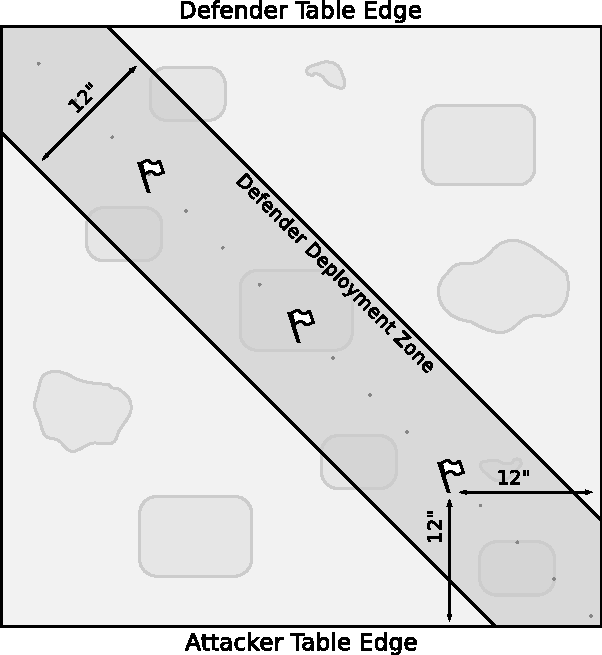
\includegraphics[width=\linewidth]{maps/mission1.pdf}}
  \end{columns}
\vspace{-2.5em}

%%----------------------------------------------
%\begin{missionrules}

\missionsubheading{Hasty Redoubts.} During deployment the Defender may
designate~3 distinct pieces of terrain at least partially in their
deployment zone.  Cover saves granted by that terrain are improved
by~1, to no better than~3+.

\missionsubheading{Sneak Attack.} During deployment the Attacker may
grant the Outflank special rule to up to~3 of their units (embarked
units do not count). After all deployment concludes, the Attacker
chooses to play first or second.

  % Defender units at least partially
  % within 3'' of the primary objective markers \emph{may} re-roll
  % failed morale checks.

%\end{missionrules}


%%----------------------------------------------
\begin{scoring}
  
\begin{primaries}

  Before any Scout redeployments, both players secretly choose one of
  the following primary scoring mechanisms for themselves:

  \begin{itemize}
  \item {\textit{Continuous.}} Beginning with Turn~2, score~1 victory
    point at the end of each of your player turns for each primary
    objective marker you control.

  \item {\textit{End Game.}} At game end, score~3 victory points for
    each primary objective marker you control.

  \end{itemize}
  This selection is declared along with the choice of secondary
  objective, below.  Remember that \underline{no more than}
  \underline{9 victory points may be earned toward primary
    objectives}.

\end{primaries}

\end{scoring}


%%----------------------------------------------------------------------
%%----------------------------------------------------------------------
\missiontitle{Mission 2: Hostility}

%\teaser{}

%%----------------------------------------------
\begin{tablesetup}
  \dawnofwar

  \bigskip%
  Place six secondary objective markers: One in each table corner~12''
  from both edges, and two more along the table centerline each~24''
  from the long edges and~27'' from a short edge.

\end{tablesetup}

%%----------------------------------------------
\begin{missionrules}

\nightfalls

\end{missionrules}


%%----------------------------------------------
\begin{scoring}
  
\begin{primaries}
  At game end, each unit that has been eliminated, is falling back, is
  in reserve, or has at most~25\% of its starting models remaining is
  broken.  Earn~2 victory points per quartile if at least 25\%, 50\%,
  and 75\% of the opposing army by units is broken.  Earn~1 victory
  point per quartile if at least 25\%, 50\%, and 75\% of your army is
  not broken.  An additional victory point is earned by the player who
  has had a smaller percentage of the units in their army broken.  If
  one player has been completely eliminated, the opposing player gains
  an additional victory point.  \underline{No more than 9 victory
    points may be earned via this primary objective.}
\end{primaries}

\begin{secondaries}
  \majoritycontrol

  \holdthefield

  \seizeground

  \assassination
\end{secondaries}

\end{scoring}


%%%----------------------------------------------------------------------
%%----------------------------------------------------------------------
\missiontitle{Mission 3: Madness}

%\teaser{}

%%----------------------------------------------
\begin{tablesetup}

\vanguardstrike

\bigskip%
After determining deployment zones, place two primary objective
markers each 18'' from a short table edge and 24'' from the long
edges.  Players then roll off on~D6 and in that order alternate
placing a total of four more objective markers.  Each player must
place their first marker in their opponent's deployment zone and their
second in their own deployment zone.  Label all of the markers~1
through~6 in any fashion.
\end{tablesetup}


%%----------------------------------------------
\begin{missionrules}

\nightfighting

\standingorders

\end{missionrules}


%%----------------------------------------------
\begin{scoring}
  
\begin{primaries}
\maelstromscoring
\end{primaries}

\pagebreak

\begin{secondaries}
  \holdthefield

  \breachpoints

  \breaktheirback

  \seekanddestroy
\end{secondaries}

\end{scoring}


%\input{tactical-sheets}

\end{document}

%%----------------------------------------------------------------------
%%----------------------------------------------------------------------

\clearpage

\noindent\begin{minipage}[t][\textheight-6pt][t]{1.0\linewidth}
\vfill  
\centerline{\Huge\emph{Missions will be posted shortly.}}
\vfill
\vbox to 0pt{}
\end{minipage}








\pagetitle{Mission Pack}

\begin{columns}

\missionheading{Army Construction}

Armies must be selected to at most~\underline{750 points}.




\missionheading{Restrictions}

Players will use a single army list for all missions.  No requirements
or constraints are placed on detachments or force organizations beyond
those listed above.  All up to date sources\footnote{Partial list
  maintained by Redcap's Corner and PAGE: \url{http://bit.ly/1uWkFHz}}
are permitted.  Forge World units and armies eligible for standard
\emph{Warhammer 40,000} are permitted.

Models need not be painted, but objective painting scores will be
applied to reward finished armies.

Models must be WYSIWYG, but identifiable and thoughtful conversions
and proxies are welcome.  Contact the tournament organizer(s)
beforehand about any uncertain models.  Indistinguishable or confusing
proxies are not permitted.

\missionheading{Supporting Materials}

You must have an official, legal, complete physical or digital copy on
hand for all army, unit, and other sources you are using.  You should
bring printed copies of relevant pages of any electronic sources.
Don't forget errata and FAQs for your sources.\footnote{Available from
  Games Workshop:
  \url{http://www.games-workshop.com/Rules-Errata}}

You must bring any dice, templates, and markers you need to facilitate
playing your army, as well two typed copies of each of your lists,
with points noted.

For any codex or supplement released within two weeks preceding the
event, players may choose whether to use the old or new edition.  They
may not use both editions of a single source within the event, e.g.,
allying old with new.

%\vfill
%\begin{story}{62pt}{The Shift}
%\end{story}
%\columnbreak

\missionheading{Scoring}%

Match results are determined by scoring primary, secondary, and
tertiary objectives as given for each mission.  The winner is the
player with more victory points at game end.  Players draw if they
have earned equal victory points.  No more than~20 victory points may
be earned per mission.

Pure competition standings, i.e., the Best General prize(s) if
awarded, are determined first by win/draw/loss records and then the
sum total victory points earned across all three missions.

Overall tournament rankings and the primary prize(s) are based on
points earned toward a maximum of~100 available for the day:
\begin{itemize}\shortlist
\item 60 points for match results
\item 25 points for painting and craftsmanship
\item 15 points for sportsmanship
\end{itemize}

Match results are a simple sum of the victory points earned in each
mission, up to 20 points each.

Painting and craftsmanship is scored objectively by the judge(s)
applying this rubric to the armies:

\begin{itemize}\shortlist
\item All models assembled and primed: +5 pts
\item All models three-color minimum: +5 pts
\item All models based (paint/flock): +5 pts
\item Advanced painting techniques present (washes, drybrushing, etc): +5 pts
\item Advanced basing techniques present: +5 pts
\end{itemize}

Sportsmanship scores include two components:
\begin{itemize}\shortlist
\item The sum of sportsmanship scores given after each mission (9 pts
  available).

\item Players ranking their opponents by most enjoyable to play (6 pts
  available).
\end{itemize}

Please make sure to submit sportsmanship scores as appropriate,
including the final ranking, as otherwise it impairs your opponents'
overall scores!

\end{columns}
